\subsection{The complete projection when finite cycling is allowed}
\label{sec:fulllossyprojection}
An exact projection can retain the otherwise dominated cycling actions.
We now explicitly permit any finite number of early charge/discharge
actions on a bus. There is no switching time, minimum session, separate
throughput fee, degradation cost or cycle limit. Common connector powers
are admissible in both directions for every bus, and all buses remain
available throughout the early window. Assume $B>0$ and a nonempty used
fleet. Economic objectives in this subsection depend on period-aggregate
loads and vehicle cost, rather than the timing or number of switches.
These assumptions are essential to the full-set claim.

\begin{theorem}[Complete common-loss load--cost projection]
\label{thm:fulllossyprojection}
For matching cardinality $m=0,\ldots,\nu$, let $N_m=2n-m$ and let
$r_m$ be the least total early battery requirement among allowed
matchings of size $m$. Define the compact polygon, possibly empty,
\begin{equation}\label{eq:fulllossypolygon}
\begin{split}
 W_m=\bigl\{(C,X):\;&C\ge r_m/\alpha,\quad X\ge0,\quad C+X\le K,\\
 &\max\{S-N_mB,S-\alpha H\}
       \le Q=\alpha C-X/\delta\le P\bigr\}.
\end{split}
\end{equation}
The complete physical load--cost projection is exactly
\[
 \bigcup_{m=0}^{\nu}
 \left\{\left(C-X,\frac{S-Q}{\alpha},fN_m\right):(C,X)\in W_m\right\}.
\]
Every point is attained by a finite-action schedule. Thus arbitrary
economic objective values on these projected quantities, including
negative posted-price value queries, are preserved without a monotonicity
assumption. Each nonempty polygon has at most five vertices; their affine
images generate the complete-plan convex hull with at most
$5(\nu+1)$ records, including lossless or lower-dimensional degeneracies.
\end{theorem}

\begin{proof}
Fix one matching, with fleet $N$, summed requirement $R$ and
$T=S-NB$. Let $x_v$ be a bus's net early battery increment.
Its paired, A-only and B-only endpoint boxes are respectively
\[
 [a_i+b_j-B,a_i],\qquad[a_i-B,a_i],\qquad[b_j-B,0].
\]
Their lower endpoints sum to $T$, their positive lower endpoints to $R$,
and their upper endpoints to $P$. Every upper endpoint is nonnegative.
Regardless of action order, $x_v=\alpha C_v-X_v/\delta$, so total
$Q\in[T,P]$. A positive lower endpoint requires at least its value
divided by $\alpha$ in purchases. Hence $C\ge R/\alpha$ is necessary.
The other inequalities are nonnegative exports, shared gross use and
full-terminal accounting $L=(S-Q)/\alpha\le H$. Terminal purchases are
nonnegative because $Q\le P<S$; individually each box upper endpoint
also leaves a nonnegative refill requirement.

Conversely fix aggregate totals satisfying these inequalities with $R$
in place of $r_m$. For any $Q\in[T,P]$, the boxes admit an exchange
vector whose positive parts sum to $A=\max\{R,Q\}$. If $Q\ge R$,
start from positive lower endpoints and zero elsewhere, distributing
$Q-R$ through the remaining headrooms. If $Q<R$, keep mandatory positive
increments and distribute negative increments of total $Q-R$ through the
negative lower intervals, whose combined lower endpoint is $T-R$.
One-direction exchanges then realize
\[
 C_0=A/\alpha,\qquad X_0=\delta(A-Q).
\]
Since $X\ge0$ implies $\alpha C\ge Q$, and
$\alpha C\ge R$, we have $z=C-C_0\ge0$ and
$X-X_0=\alpha\delta z$.

Realize these residuals by battery-neutral cycles on one existing bus
before its one-direction exchange. At early SOC $s\in[0,B]$, use
charge-then-discharge cycles of depth at most $B-s$ if $s\le B/2$,
and discharge-then-charge cycles of depth at most $s$ otherwise.
The permitted depth is at least $B/2>0$. Split the residual battery
throughput $\alpha z$ into finitely many such chunks, allowing a smaller
last chunk. Each returns to $s$, stays in $[0,B]$, and uses grid purchases
depth$/\alpha$ and exports $\delta$ times depth. Their total residual
is exactly $(z,\alpha\delta z)$, with no limiting or Zeno argument.

Execute the cycles and then all one-direction exchanges serially.
Their gross grid throughput is exactly $C+X\le K$, so they fit the
common early window at the admitted power. Endpoint boxes ensure
subsequent service feasibility; nonnegative service consumption preserves
intermediate SOC. Refill serially at the terminal, using total
$L\le H$. If $K=0$, all early actions are zero and no positive-power
division is required. If $H=0$, only zero terminal amounts could be
admitted; under the present positive B-service energies, $P<S$ makes
every polygon empty, consistently with physical infeasibility.

At fixed $m$, only $R$ depends on the matching: $S,P,N,T$ and the fee
are constant. Its entire polygon is contained in the polygon for a
matching attaining $r_m$, and every point of that larger polygon has
just been physically constructed. This proves exact equality of the
union, not merely economic dominance. Equation~\eqref{eq:fulllossypolygon}
has five halfspaces in the plane. Its bounded polygon has at most five
vertices; affine images and then finite convex combinations prove the
generator claim. When $\alpha\delta=1$, the map collapses to
$E+L=S/\alpha$ rather than being invertible; the same argument still
applies.
\end{proof}

\begin{corollary}[Capped identical idle buses in the complete projection]
Under the same zero-transition model, permitting identical paid idle buses
with a total fleet cap $2n$ leaves this complete projection unchanged.
\end{corollary}
An idle bus has exchange box $[-B,0]$. A fleet with matching size $m$ and
$q$ idle buses has $q\le m$ by the cap. Delete $q$ matching edges and
serve their services separately. This preserves total $N,S,P,T$ and fee,
while lowering $R$. The resulting all-assigned polygon reproduces the same
$C,X,Q,E,L,c$, including cycles. Reverse inclusion is immediate. Identical
access, efficiency, capacity and fees are required; nonzero transition
consumption would change $S$ under deletion and needs a separate argument.

Let $V$ be the vertex-image records in the theorem. An exact continuous
formulation for complete-plan convexification is the familiar relation
\[
 \operatorname{conv}\mathcal P
   =\left\{\sum_{v\in V}\lambda_vv:
          \lambda_v\ge0,\ \sum_{v\in V}\lambda_v=1\right\},
\]
where $\mathcal P$ denotes the complete projected set above. A convex
$F$ gives ordinary convex planning on each polygon and on this hull;
physical planning takes the minimum over the cardinalities. These are
standard convex-optimization tools. Merely interpolating $r_m$ at a
fractional cardinality and substituting into physical inequalities is
not this disjunctive hull construction and remains unjustified.

Removing a neutral cycle keeps $Q,L$ fixed and lowers $E$ by
$(1-\alpha\delta)z$. This explains why monotone objectives can discard
it in the efficient-frontier result below, while arbitrary objectives
must retain the full polygons. Its smaller set $Z$ still requires the
stated monotonicity assumptions. The finite cycle count can be large;
no runtime or generic hull-algorithm claim is made. A separate eight-case
exact qualification of these full polygons, described in
Appendix~\ref{app:evidence}, includes finite-action physical replay.
It supplies no public-timetable V2G, empirical or learning evidence.
The earlier one-direction qualification has a different scope.

\paragraph{Why a negative-price query needs the full set.}
Take $n=1$, $B=1$, $a=b=3/4$, $\alpha=1/2$, $\delta=1$,
$K=2$, $H=3$ and $f=2$. At the fixed posted prices $p=(-3,1)$,
the private score is $c-3E+L$. For the paired one-bus assignment,
\[
 C=11/6,\quad X=1/6,\quad Q=3/4,
 \qquad (E,L,c)=(5/3,3/2,2)
\]
gives score $-3/2$. This point has a finite physical realization.
After A the battery holds $1/4$: purchase $1/3$ grid units and export
$1/6$, returning to $1/4$, then purchase $3/2$ to reach full.
These three early actions have gross energy 2 and serialize at power 2
within the early window. B leaves $1/4$; terminal purchases $3/2$
restore full inventory within the power-3 terminal window.

This is the exact response value, not just a feasible score.
For $m=1$, the polygon has $C\ge1$ and
$1/2\le C/2-X\le3/4$; for $m=0$, it has $C\ge0$ and
$0\le C/2-X\le3/4$. Both impose $X\ge0$ and $C+X\le2$.
Their scores are respectively $5-4C+5X$ and $7-4C+5X$.
For any feasible $C$, use the smallest export
$X=\max\{0,C/2-3/4\}$. The resulting score decreases on both
pieces, with final endpoint $C=11/6$, giving minima $-3/2$ and
$1/2$, respectively. Thus the complete-fleet response value is $-3/2$.

The efficient curves instead have $L=3-E$: the two-bus curve has
$0\le E\le3/2$, $c=4$, and the one-bus curve has
$1\le E\le3/2$, $c=2$. Their best scores are 1 and $-1$.
Discarding the neutral cycle therefore changes this query's value from
$-3/2$ to $-1$. It raises early purchases without changing terminal
refill, so the negative early rate rewards a point that monotone
economics discards. Because the queried objective is linear, its minimum
over the physical set and its complete-plan hull is the same:
$D=\CH=-3/2$ for this objective. This is not a positive planning gap
or an equilibrium claim. This analytical anchor also passed the separate
full-polygon implementation control; it gives no public-timetable V2G conclusion.

\begin{figure}[htbp]
\centering
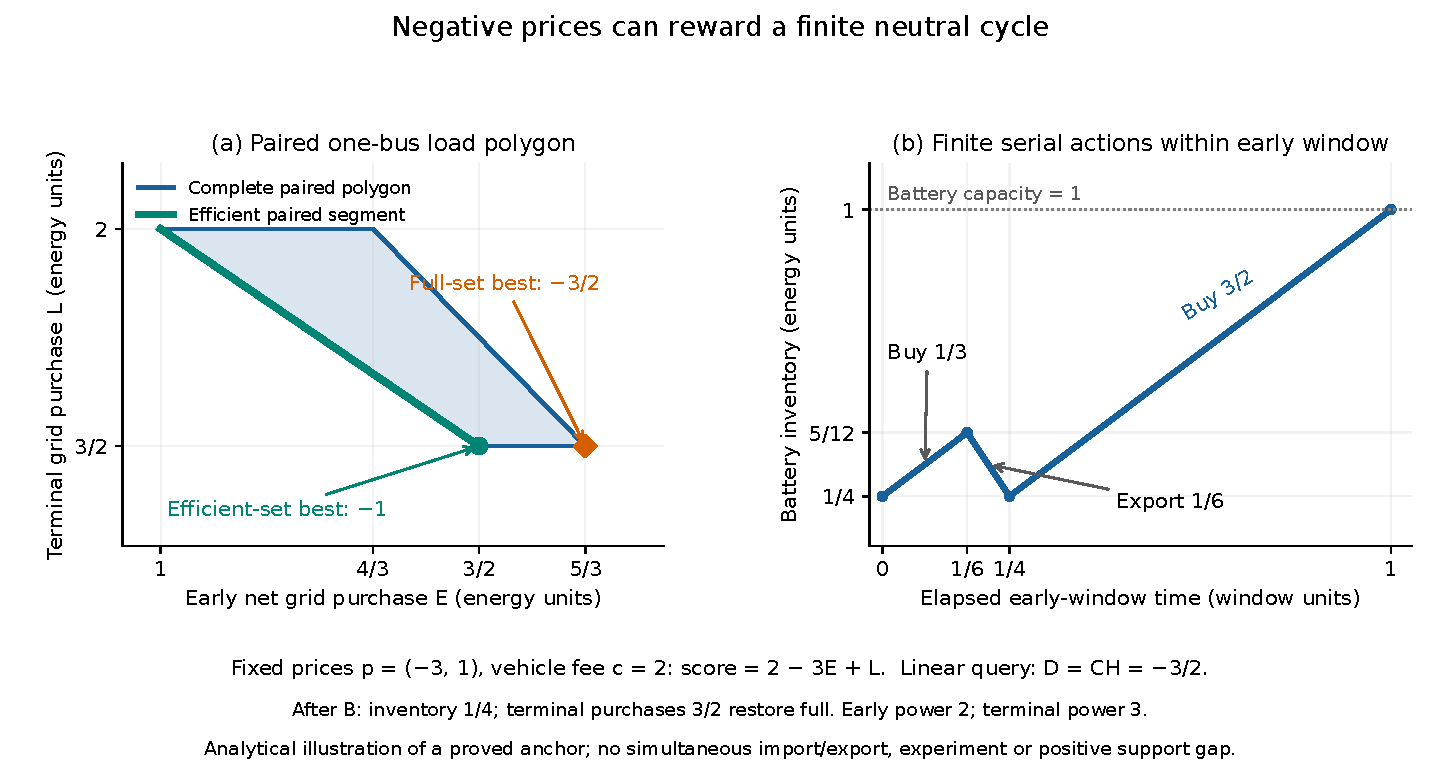
\includegraphics[width=\textwidth]{figures/full_lossy_polygon-v2.pdf}
\caption{The full paired polygon retains a finite neutral cycle that the
efficient frontier discards. At the negative posted price, that cycle improves
the fleet's linear response value. This illustration has $D=\CH$; it is not a
positive planning-gap example. The right panel shows the three serial early
actions of the same physical witness.}
\label{fig:fullpolygon}
\end{figure}

\begin{corollary}[Directional powers, affine wear and a finite action cap]
\label{cor:directionalwear}
Retain the full-action assumptions of
Theorem~\ref{thm:fulllossyprojection}. In the unit early window let common
purchase power be $K_c>0$ and export power $K_d>0$, accepted by every
bus in the corresponding direction. Replace the gross-budget halfspace by
\[
 C/K_c+X/K_d\le1.
\]
With the other four halfspaces unchanged, these are still the exact
cardinality polygons. For common affine grid-throughput wear coefficients,
their complete joint load--cost images are
\[
 E=C-X,\qquad L=(S-Q)/\alpha,\qquad
 c=fN_m+w_cC+w_dX+w_tL.
\]
Each polygon still has at most five vertices, whose affine images generate
the complete-plan hull. Fixed nonnegative wear coefficients have their
usual cost interpretation; exact projection equality itself needs no
coefficient-sign or economic-monotonicity restriction.

For a fixed used fleet $N$, every attainable aggregate point has a
realization with at most
\[
 N+2\left\lceil\frac{2\alpha K_c}{B}\right\rceil
 \quad\hbox{early charge/export actions},\qquad
 N\quad\hbox{terminal charge actions}.
\]
An action cap at least these bounds preserves the aggregate projection,
not every literal schedule. Replacing $N$ by $2n$ gives one bound for
all cardinalities under the standing fleet cap.
\end{corollary}

\begin{proof}
The endpoint boxes, mandatory purchases and terminal accounting are
unchanged. Necessity of the new halfspace follows because the two
directions occupy at least $C/K_c$ and $X/K_d$ connector time and cannot
overlap. For sufficiency use the same baseline exchanges and neutral
cycles as in Theorem~\ref{thm:fulllossyprojection}. Execute each purchase
at power $K_c$ and each export at $K_d$; their total serial duration is
exactly the displayed occupancy. Directional asymmetry adds no SOC
condition. At fixed cardinality a minimum-$R$ matching reproduces the
same $C,X,Q,L$, hence the same affine wear cost, for any other matching.
This proves complete-set equality; affine imaging and convex combination
give the vertex and hull claims. The common-task version uses $S_m$
in place of $S$, as in Corollary~\ref{cor:commontransitionfull}.

The residual $z=C-C_0$ has battery throughput $\alpha z\le\alpha K_c$.
Choosing chunks of depth $B/2$, with a possibly smaller last chunk, needs at most
$J=\lceil2\alpha K_c/B\rceil$ cycles, each with two actions. The chosen
orientation fits the bus's initial SOC, and each cycle returns to it.
Each bus then needs at most one baseline early action and one terminal
charge; zero actions are omitted. Restricting to this action count adds
no aggregate point and removes none, since every point has the explicit
bounded-action realization. The count is conservative, not minimal,
and does not bound runtime or the number of actions in arbitrary schedules.
\end{proof}

Wear must remain in the cost image. In the lossless case a neutral cycle
adds equal amounts $z$ to $C,X$, leaving $E,L$ unchanged but adding
$(w_c+w_d)z$ to intrinsic cost. Thus net loads and a constant vehicle
fee alone cannot represent this complete joint projection. For the same
reason, convexification retains each component's actual wear cost. Affine
wear commutes with averaging when $C,X,L$ remain separate; mean net loads
alone need not determine it.

This corollary does not transfer the smaller efficient-$Z$ formulas to
unequal powers or wear, nor cover SOC/depth/rate-dependent degradation,
per-session cost, positive switching time, minimum durations or
heterogeneous acceptance. Its positive-power assumptions are separate
from the theorem's zero-budget cases. It is an analytical extension with
no numerical implementation qualification: the eight full-polygon cases
use symmetric early powers and no wear. No public-timetable, empirical
wear-calibration or computational-advantage conclusion follows.
